%%%%%%%%%%%%%%%%%%%%%%%%%%%%%%%%%%%%%%%%%%%%%%%%%%%%%%%%%%%%%%%%%%%%%%%%%%
%%%%%                         CHAPITRE 1                            %%%%%%
%%%%%%%%%%%%%%%%%%%%%%%%%%%%%%%%%%%%%%%%%%%%%%%%%%%%%%%%%%%%%%%%%%%%%%%%%%

\lhead[\fancyplain{}{\leftmark}]%Pour les pages paires \bfseries
{\fancyplain{}{}} %Pour les pages impaires
\chead[\fancyplain{}{}]%
{\fancyplain{}{}}
\rhead[\fancyplain{}{}]%Pour les pages paires 
{\fancyplain{}{\rightmark}}%Pour les pages impaires \bfseries
\lfoot[\fancyplain{}{}]%
{\fancyplain{}{}}
\cfoot[\fancyplain{}{\thepage}]%\bfseries
{\fancyplain{}{\thepage}} %\bfseries
\rfoot[\fancyplain{}{}]%
{\fancyplain{}{\scriptsize}}


%%%%%%%%%%%%%%%%%%%%%%%%%%%%%%%%%%%%%%%%%%%%%%%%%%%%%%%%%%%%%%%%%%%%%%%%%%
%%%%%                      Start part here                          %%%%%%
%%%%%%%%%%%%%%%%%%%%%%%%%%%%%%%%%%%%%%%%%%%%%%%%%%%%%%%%%%%%%%%%%%%%%%%%%%

\adjustmtc % jouer avec adjustmtc (ajuster minitoc si problème dans la numérotation)

\chapter{Titre 1}
\label{ch:1}

%==============================================================================	Résumé du chapitre

\begin{center}
	\rule{0.7\linewidth}{.5pt}
	\begin{minipage}{0.7\linewidth}
		\smallskip
		
		\textit{Résumé du chapitre possible ici.
		}
		
		%\smallskip
	\end{minipage}
	\smallskip
	\rule{0.7\linewidth}{.5pt}
\end{center}

\minitoc
\newpage

\section{Introduction}
\label{Ch1:S:intro}

Introduction

Tout le mérite de ce document revient au SYMME et à Jean Collomb bien pûr.

\section{Citations et références}
\label{Ch1:S:citations et references}

\subsection{Citations}

En utilisant apalike, les citations peuvent être données directement dans le text comme avec \cite{Reiersol1950}.

Une citation peut être donnée entre parenthèse aussi \citep{Reiersol1950}.

Même chose avec plusieurs citations \cite{Reiersol1950,Walter1994b} ou entre parenthèse \citep{Reiersol1950,Walter1994b}.

Astuce : demander à Mendeley de créer une mise à jour automatique de toutes les citations dans un library.bib qu'on fait enregistrer automatiquement dans le dossier Fichiers\_latex/Ref/. Le fichier Biblio fait référence à ce fichier.

\subsection{Références}

Et hop une référence à l'introduction \ref{Ch1:S:intro}.

\begin{sloppypar}
	On peut faire apparaître les références en noir ou en une autre couleur en allant dans fichiers\_latex/Manuscrit/Packages.tex, à la fin du fichier dans les options de hyperref.
\end{sloppypar}

\section{Les figures}
\label{Ch1:S:figures}

On changera dans manuscrit.tex la façon d'appeler les figures et les tableaux (Fig. au lieu de Figure, Tableau ou Tab. au lieu de Table).

On peut intégrer des figures simples comme \ref{Ch1:fig:simple} ou \ref{Ch1:fig:simple frac}, dont la taille est automatiquement de la largeur du texte. Le mieux est d'enregistrer les figures en pdf, elles sont vectorisées et c'est moins casse-pied que d'intégrer des svg.

\begin{figure}
	\centering
	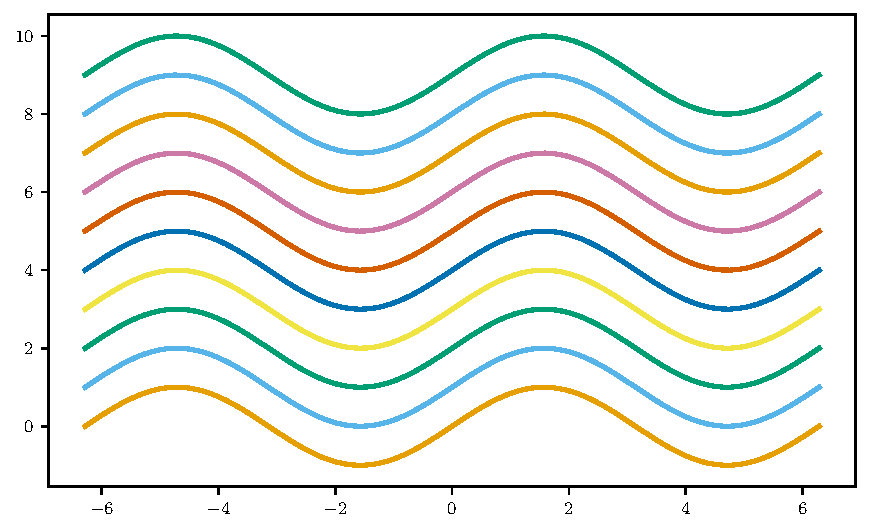
\includegraphics{../Chap1/Figure/Figure_simple_largeur_max.pdf}
	\caption{Légende de la figure. On remarque que le cycler des couleurs tourne en rond au bout de 7 couleurs. Les couleurs sont ok pour les daltoniens (true story!). This size is the default size of the set\_size python function in the notebook.}
	\label{Ch1:fig:simple}
\end{figure}

\begin{figure}
	\centering
	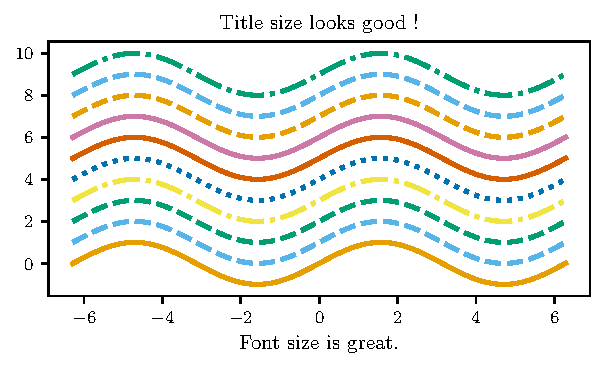
\includegraphics{../Chap1/Figure/Figure_simple_fraction.pdf}
	\caption{On peut varier automatiquement le linestyle aussi, ça rend mieux pour distinguer les couleurs. La taille peut être réglée automatiquement à une fraction de la taille précédente.}
	\label{Ch1:fig:simple frac}
\end{figure}

Ou figures avec sous-figures. On cite la sous-figure \ref{Ch1:fig:multiple1} ou la figure totale \ref{Ch1:fig:multiple}.

\begin{figure}
	\centering
	\begin{subfigure}[b]{\textwidth}
		\centering
		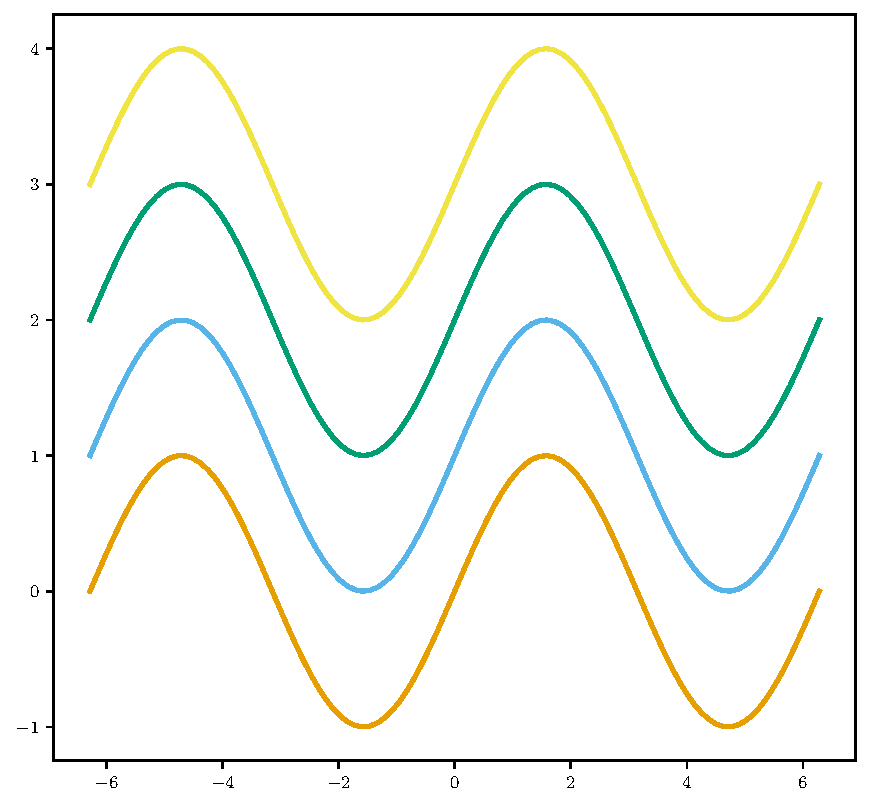
\includegraphics{../Chap1/Figure/Figure_simple_larger_height.pdf}
		\caption{Larger height, full text width}
		\label{Ch1:fig:multiple1}
	\end{subfigure}
	%	\vspace{8pt}
	\begin{subfigure}[b]{\textwidth}
		\centering
		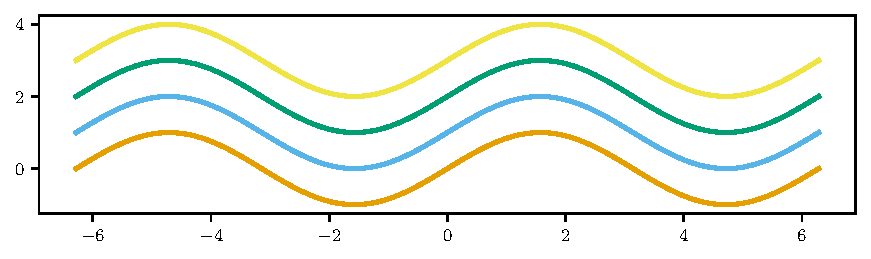
\includegraphics{../Chap1/Figure/Figure_simple_smaller_height.pdf}
		\caption{Smaller height, full text width}
		\label{Ch1:fig:multiple2}
	\end{subfigure}
	\caption{This multiple figure is so high that latex reserves a full page for display (as soon as figure > 0.75 height page). It is a parameter that can be changed somewhere in meta-class...}
	\label{Ch1:fig:multiple}
\end{figure}

Figures with multiple subplots with matplotlib directly have no individual labels to be referred to, which is sometimes just fine, see \ref{Ch1:fig:multiple matplotlib 21} or \ref{Ch1:fig:multiple matplotlib 12}.

\begin{figure}
	\centering
	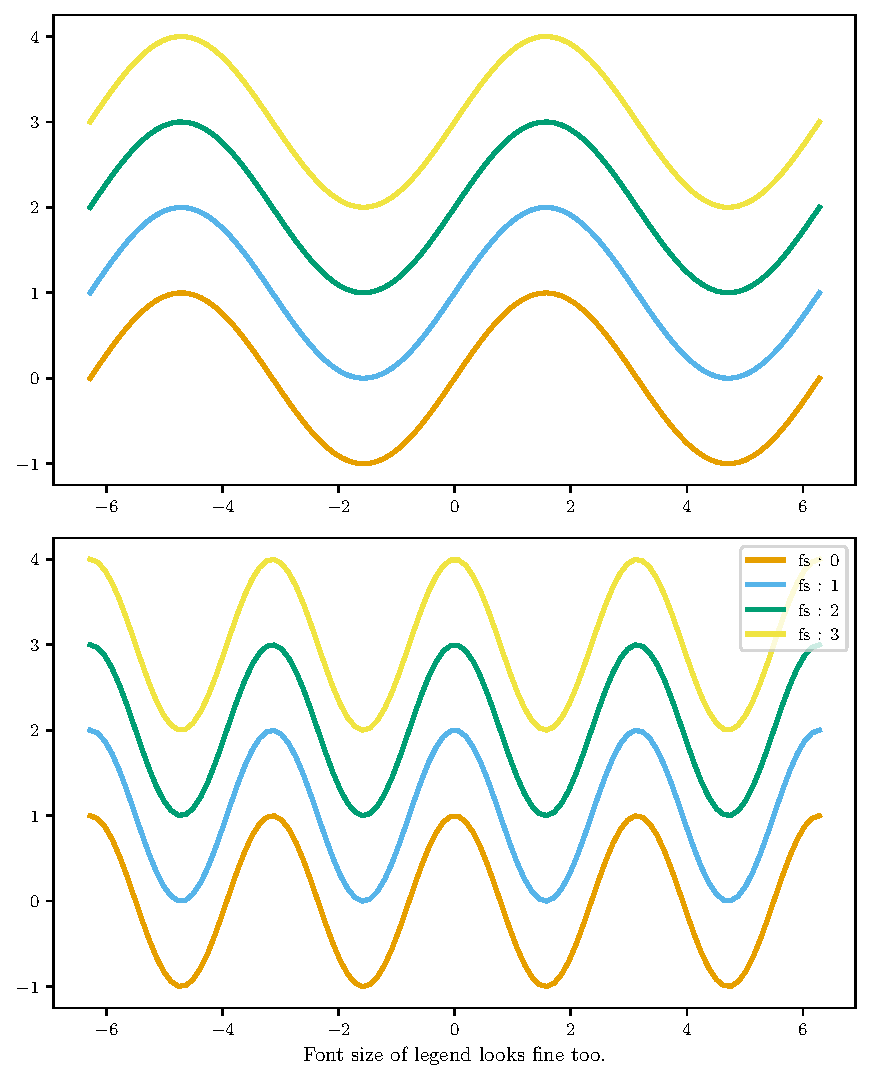
\includegraphics{../Chap1/Figure/Figure_multiple_21.pdf}
	\caption{Multiple subplots with matplotlib is also possible, with output at perfect width for this manuscript template. There is no individual legend possible...}
	\label{Ch1:fig:multiple matplotlib 21}
\end{figure}

\begin{figure}
	\centering
	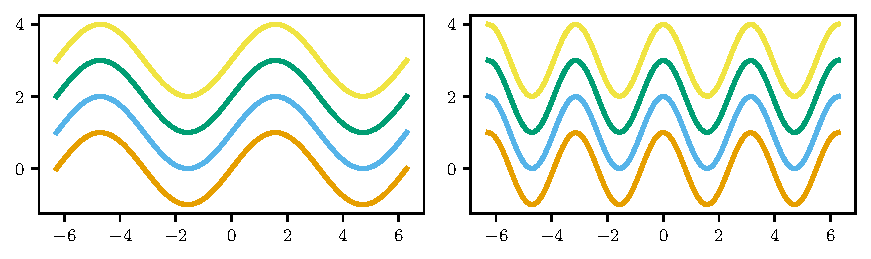
\includegraphics{../Chap1/Figure/Figure_multiple_12.pdf}
	\caption{Another example of matplotlib subplots}
	\label{Ch1:fig:multiple matplotlib 12}
\end{figure}

\FloatBarrier % sert à éviter que les figures partent dans les sections suivantes.

Ci-dessous on a crée un type de float qui porte un nom différent (pas juste une figure ou un tableau) qui s'appelle donc Model, qui a sa propre numérotation \ref{Ch2:mod:nom du modele} , et ce cite avec par exemple \autoref{Ch2:mod:nom du modele}.

\begin{modelfloat}
	\begin{center}
		\begin{circuitikz}
			\draw
			(0,0) to [short] (4,0)
			(4,2) node[circ]{}
			to [R, l=$R$] (0,2)
			to [ceV, l_=$T_e$] (0,0)
			(2,0) node[ground] {}
			(4,0) to [C, l=$C$] (4,2)
			{[anchor=south] (4,2) node {$T_i$} (6,2)}
			;
		\end{circuitikz}
	\end{center}
	\[
	\left\{
	\begin{array}{ c c l }
	\dot{T_i} 
	&
	=
	&
	- \frac{1}{CR}
	T_i
	+
	\frac{1}{CR}
	T_e
	\\
	y
	&
	=
	&
	T_i
	\end{array}
	\right.
	\]
	\caption{This custom float has a first part RC model with circuitikz and its equations.}
	\label{Ch2:mod:nom du modele}
\end{modelfloat}


\FloatBarrier % sert à éviter que les figures partent dans les sections suivantes.

\section{Du code joli}

\begin{lstlisting}[frame=single, numbers=right, rulecolor=\color{myblue3}]
MODEL EQUATION(S)
c_ := {df(ti,t)=(text - ti + ga*isol*r)/(c*r),y=ti}

CHARACTERISTIC SET
aa_(1) := df(y,t)*c*r - isol*ga*r - text + y
aa_(2) :=  - ti + y

MODEL ALGEBRAICALLY OBSERVABLE

PARAMETER VALUES
b2_ := {c=2,r=3,ga=5}

MODEL PARAMETER SOLUTION(S)
g_ := {{c=(2*ga)/5,r=15/ga}}

MODEL NON IDENTIFIABLE
\end{lstlisting}

\section{Des tableaux}

\begin{table}[]
	\centering
	\begin{tabular}{c|c|}
		\cline{2-2}
		& Crest Factor \\ \hline
		\multicolumn{1}{|c|}{Diffuse solar irradiation}              & 4.93         \\ \hline
		\multicolumn{1}{|c|}{Global horizontal irradiation}          & 3.24         \\ \hline
		\multicolumn{1}{|c|}{Global vertical south irradiation} & 2.72         \\ \hline
	\end{tabular}
	\caption{Légende du tableau}
	\label{Ch2:tab:crest_solar}
\end{table}

Générateur en ligne \href{http://www.tablesgenerator.com/latex_tables}{ici}. \\

Un exemple de tableau générée par cet outil est présenté Table~\ref{Ch1:tab:exemple}.

\begin{table}[]
	\centering
	\begin{tabular}{c|c|c|c|}
		\cline{2-4}
		& \textbf{A}                 & \textbf{B} & \textbf{C} \\ \hline
		\multicolumn{1}{|c|}{$\alpha$} & \multicolumn{3}{c|}{\textit{fusion}}                 \\ \hline
		\multicolumn{1}{|c|}{$\beta$}  & \multirow{2}{*}{\textit{}} & \textit{1} & \textit{2} \\ \cline{1-1} \cline{3-4} 
		\multicolumn{1}{|c|}{$\Delta$} &                            & \textit{3} & \textit{4} \\ \hline
	\end{tabular}
	\caption{Exemple de tableau}
	\label{Ch1:tab:exemple}
\end{table}

\section{Conclusion}

Une conclusion
